\documentclass[11pt]{article}
\usepackage{graphicx}       
\usepackage{caption}
\usepackage{hyperref}
\hypersetup{
    colorlinks=true,
    linkcolor=blue,
    filecolor=magenta,      
    urlcolor=cyan,
}
\usepackage{mathtools}\usepackage{tkz-euclide}\usepackage{amsmath}
\usepackage{xepersian}
\settextfont[Scale=1.1]{XB Yas}
\title{%
به نام خدا%
\\[1cm]
مستند اپلیکیشن یادمان}
\author{تیم برنامه‌نویسی:\\
محمد امین سالارکیا\\
   مهدی قنبری\\
   محمد تابع امام\\
   امیرحسین مهدی‌نژاد\\
   امیر سده}
\date{۱۳۹۶/۱۲/۱۶}
\begin{document}

\maketitle

\section{مقدمه}

اپلیکیشن یادمان نرم‌افزاری جهت یادگیری آسان دروس حفظی کنکور به روش لایتنر است. در این اپلیکیشن با استفاده از دیتابیس جامعی از دروس حفظی کنکور دانش‌آموز با اضافه کردن کارت به جعبه لایتنرش میتواند دروس را مرور کند. مخاطب این اپلیکیشن تمام دانش‌آموزان دبیرستانی و به خصوص کنکوری‌ها هستند.\par
در این مستند سعی شده تمام کدهای پیاده‌سازی شده و بخش‌های اپلیکیشن توضیح داده شود. ابتدا طراحی مدل‌های برنامه و دیتابیس توضیح داده شده و سپس ماژول‌های برنامه آورده شده.کد‌های اپلیکیشن را میتوانید در 
\href{https://github.com/M-amin-s/Yademan}{این مخزن}
ببینید.

\section{طراحی مدل‌ها و دیتابیس}
نمودار uml مدل‌ها را در شکل ۱ میتوانید ببینید.\\\\\\
\begin{figure}[h]
    \centering
    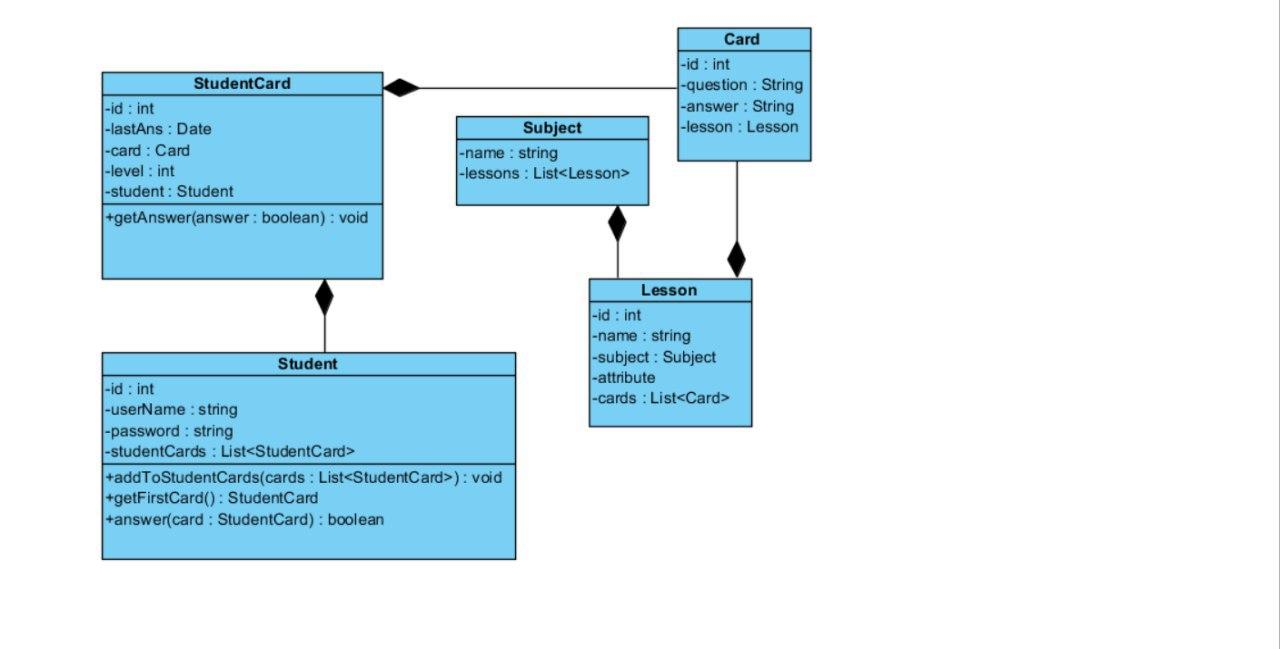
\includegraphics[width=1.5\textwidth]{uml_diagram}
    \caption{نمودار uml مدل‌ها}
    \label{شکل:نمودار uml}
\end{figure}

مدل \lr{StudentCard} نشان‌دهنده کارت‌های اضافه شده به جعبه است.\\ مدل‌های
\lr{Subject, Lesson, Card}
 مربوط به دیتابیس استاتیک بوده و به ترتیب مبحث(ادبیات، زبان،...)،درس(درس یک، درس دو، ...) و کارت‌های هر درس هستند.\\
 
 به غیر از این مد‌ل‌ها مدل‌های دیگری هم(مثل \lr{Notification, QueueObject,Quiz,...} ) برای پیاده‌سازی ماژول‌های مختلف ساخته شده که در توضیح همان ماژول آورده شده.
 
 
\section{ماژول‌ها}
تمام فایل‌های برنامه در فولدر‌های 
\lr{activities, database, models, ui, utils} 
پیاده‌سازی شده. در فولدر \lr{ui} فایل‌های مربوط به رابط کاربری(دیالوگ‌ها، لیست‌ها، کنترل فونت و ...) قرار داده شده. در فولدر \lr{database} هم فایل‌های مربوط به خواندن، اضافه کردن، آپدیت کردن و پاک کردن مدل‌ها از دیتابیس برنامه قرار داده شده.\\
در ادامه ماژول‌های برنامه آورده شده که فایل‌های مربوط به هر ماژول توضیح داده شده. این فایل‌ها در یکی از پنج فولدر بالا قرار دارند.
\subsection{ورود و ثبت‌نام و خروج}
فایل‌های مربوطه:\\
\begin{latin}
LoginActivity, EmailSignUpActivity, SignUpActivity, SignUpDetailsActivity, VerificationActivity, Connection, SharedPreferencesHandler, ConnectionUi\\
\end{latin}

ماژول ورود و ثبت‌نام از طریق سرور اولین ماژولی است که کاربر با آن مواجه میشود. \\
تمام ارتباط‌ها با سرور از طریق کلاس \lr{Connection} انجام میشود. واسط کاربری در حین ارتباط‌ها با سرور در \lr{ConnectionUi} پیاده‌سازی شده.\\
 ابتدا کاربر وارد \lr{LoginActivity} میشود برای ورود. در صورت کلیک بر روی گزینه ثبت‌نام وارد \lr{SignUpActivity} میشود برای ثبت‌نام. بعد از وارد کردن شماره تلفن وارد صفحه \lr{VerificationActivity} میشود و بعد از تایید شماره تلفن وارد \lr{SignUpDetailsActivity} میشود برای تکمیل اطلاعات ثبت‌نام. اگر کاربر بخواهد از طریق ایمیل ثبت‌نام کند (نه شماره تلفن) وارد صفحه \lr{EmailSignUpActivity} میشود. \\
اطلاعات کاربر وارد شده در \lr{cache} برنامه ذخیره میشود که این کار از طریق \lr{SharedPreferencesHandler} انجام میشود.

\subsection{شروع کار}
فایل‌های مربوطه:\\
\begin{latin}
FirstPageActivity, HomeActivity, DatabaseDownloader, FileDownloader, TutorialViewer\\
\end{latin}

در اولین بار ورود کاربر فایل دیتابیس دروس دانلود میشود. اینکار از طریق \lr{DatabaseDownloader} و \lr{FileDownloader} انجام میشود.\\
در ضمن پس از اولین ورود آموزش استفاده از اپلیکیشن نمایش داده میشود. که این کار از طریق \lr{TutorialViewer} انجام میشود.\\
هر دفعه که اپلیکیشن باز میشود آیکون یادمان در یک صفحه برای مدت کمی نشان داده میشود که این کار در \lr{FirstPageActivtiy} انجام میشود.

\subsection{انتخاب کارت، جعبه لایتنر}
فایل‌های مربوطه:\\
\begin{latin}
SelectCardsActivity, CardActivity, ImageDownloader, DataTimeUtils, Tick\\
\end{latin}

در بخش انتخاب کارت کاربر میتواند با تیک زدن درس یا مبحث یا سال خاص و زدن دکمه تایید تعداد کارت وارد جعبه لایتنرش کند یا از آن خارج کند. این کار در \lr{SelectCardsActivity} و مدل \lr{Tick} انجام شده.\par
در بخش مرور کارت کاربر میتواند کارت‌های جعبه را با سیستم لایتنر {0, 2, 4, 8, 15} مرور کند. هر کارت یک سوال دارد که با زدن گزینه نمایش پاسخ، پاسخ آن نمایش داده میشود. این قسمت در \lr{CardActivity} پیاده‌سازی شده.\par
تاریخ‌ها به صورت میلادی در دیتابیس ذخیره میشوند. تمام کار‌های مربوط به تغییر یا تبدیل تاریخ در \lr{DateTimeUtils} پیاده سازی شده.\\
برای کارت‌هایی که عکس داشته‌ باشند هر دفعه عکس‌ها دانلود میشوند که این کار در \lr{ImageDownloader} پیاده‌سازی شده.


\subsection{فروشگاه}
فایل‌های مربوطه:\\
ماژول پرداخت درون‌برنامه‌ایِ بازار  و \lr{ShoppingActivity} \\

در بخش فروشگاه کاربر میتواند کارت‌های مربوط به مباحث مختلف را بخرد. پس از خرید که از طریق ارتباط با سرور انجام میشود درس‌های خریده شده در دیتابیس برنامه ثبت میشوند. این کار در \lr{ShoppingActivity} انجام شده. در ضمن از ماژول پرداخت درون‌برنامه‌ای بازار(\lr{com.example.android.trivialdrivesample.utill}) برای پیاده‌سازی پرداخت استفاده شده.

\subsection{آزمون‌ها}

فایل‌های مربوطه:\\
\begin{latin}
SelectCardsActivity, Quiz, QuizCenter, Connection\\
\end{latin}

دانش آموز میتواند در بخش انتخاب کارت با انتخاب آزمون‌های قلمچی، گزینه‌دو،گاج و سنجش، کارت‌های مربوط به هر آزمون را به جعبه لایتنر خود اضافه کند. دریافت اطلاعات هر آزمون از طریق سرور انجام میشود. مدل‌‌های آزمون‌ها در \lr{Quiz} و \lr{QuizCenter} پیاده‌سازی شده. انتخاب آزمون هم در \lr{SelectCardsActivity} انجام میشود. 


\subsection{اطلاع‌رسانی(Notification)}
فایل‌های مربوطه:\\
\begin{latin}
NotificationsActivity, NotificationEventReceiver, NotificationIntentService, NotificationServiceStarterReceiver, Notification\\
\end{latin}

در طول زمان سه نوع پیام به کاربر داده میشود.یک نوع پیام مربوط به یاد‌آوری مرور کارت‌ است که هر روز به کاربر داده میشود. یک نوع پیام مربوط به یاد‌آوری هماهنگ‌سازی اطلاعات با سرور است که اگر سه روز از آخرین هماهنگ‌سازی اطلاعات با سرور گذشته باشد به کاربر داده میشود. و یک نوع دیگر پیام، پیام‌ها‌ای است که در سرور در نظر گرفته میشوند (مثلا برای مناسبت‌های خاص یا تبلیغ یا ...) که برنامه هر ۶ ساعت یکبار چک میکند که اگر در سرور پیام جدیدی موجود بود به اطلاع کاربر میرساند.\par
زمانبندی و ارسال پیام در \lr{NotificationEventReceiver} و \lr{NotificationIntentService} و \lr{NotificationServiceStarterReceiver} انجام میشود.\\
در ضمن همه پیام‌ها در \lr{NotificationActivity} نشان داده میشوند. که مدل \lr{Notification} در دیتابیس ذخیره میشود و برای نشان دادن همه پیام‌ها استفاده میشود.

\subsection{هماهنگ‌سازی با سرور}

فایل‌های مربوطه:\\
\begin{latin}
HomeActivity, DataSyncer, QueueObject\\
\end{latin}

تمام کار‌های کاربر به صورت یک صف در دیتابیس داخلی از طریق مدل \lr{QueueObject} ذخیره میشود. بعد از اینکه کاربر دکمه هماهنگ‌سازی با سرور را در \lr{HomeActivity} کلیک کرد تمام این صف از طریق \lr{DataSyncer} در سرور اعمال میشود و سپس کل کارت‌های سرور در دیتابیس داخلی قرار داده میشوند.

\subsection{تنظیمات}


فایل‌های مربوطه:\\
\begin{latin}
SettingsActivity, Connection, SharedPreferencesHandler\\
\end{latin}

تنظیمات اکانت(تغییر ایمیل، تغییر رمز عبو، خروج از حساب و حذف اکانت) و اندازه فونت و تنظیمات ارسال پیام و ذخیره‌سازی عکس کار‌ت‌ها در \lr{SettingsActivity} قابل تغییر است.

\section{ایرادات و توسعه‌های آتی}
در اینجا چند ایراد که رفع آن‌ها در بهتر کردن کد موثر است آورده شده:
\begin{itemize}
\item در کار با دیتابیس میتوان از کتابخانه‌های \lr{ORM} استفاده کرد که هم به بهتر شدن کد و هم به سرعت برنامه کمک میکند.
\item در ارسال \lr{Push-Notification} میتوان از سرویس‌های آماده مانند \lr{Google Firebase} استفاده کرد.
\item هماهنگسازی اطلاعات با سرور میتواند با الگوریتم‌های بهتر و  با سرعت بالاتر انجام شود
\item بهتر است برای ماژو‌‌ل‌های مختلف \lr{Test} های مختلف نوشته شود که در این بین میتوان از سرویس ‌های تست نویسی اندروید(مانند \lr{Monkey-test} و ...) استفاده کرد.
\end{itemize}
\end{document}